\subsection{Arquitectura del cliente}

En el caso del cliente, se ha trabajado con varios frameworks: React.js \cite{react}, uno de los frameworks más populares de JavaScript para realizar clientes de aplicaciones web, y Tailwind \cite{tailwind} como framework de CSS \cite{css}, utilizado para estilizar las páginas web.
\\

En cuanto a las dependencias, estas son gestionadas por npm \cite{npm}, un gestor de paquetes para Node.js, y son indicadas en el archivo {\bf package.json}. Como principales dependencias instaladas mediante npm destacan:
\begin{itemize}
    \item {\bf React Diff Viewer \cite{reactdiffviewer}}: componente de React que permite la visualización de diferencias entre dos textos.
    \item {\bf Heroicons \cite{heroicons}}: iconografía que permite ser gestionada mediante propiedades CSS de Tailwind.
    \item {\bf Material UI \cite{materialui}}: componentes e iconografía que han sido implementados con el objetivo de un desarrollo más rápido en páginas web. También constan de integración con Tailwind.
\end{itemize}

\begin{figure}[H]
\centerline{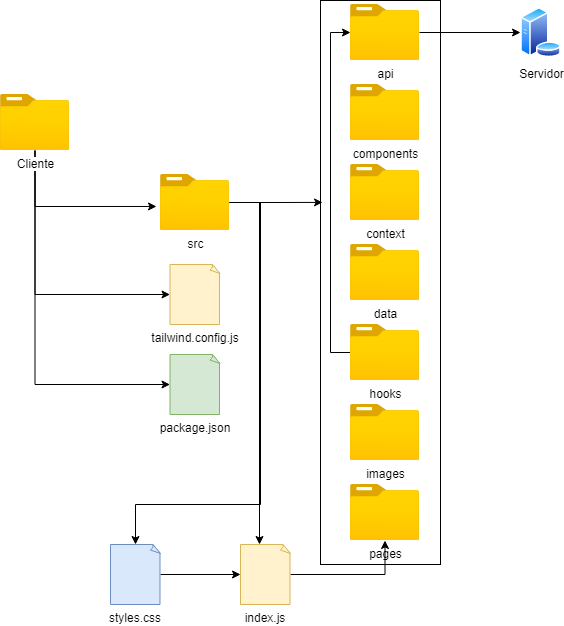
\includegraphics[width=10cm]{figuras/diseño/FicherosCliente.png}}
\caption{Arquitectura del cliente.}
\label{enlaceArquitecturaCliente}
\end{figure}

En cuanto a la arquitectura en sí, encontramos el archivo {\bf package.json} mencionado anteriormente, así como el archivo {\bf tailwind.config.js}. Este último se encarga de definir nuevas propiedades de Tailwind a la hora de aplicar el CSS sobre la página.
\\

En la carpeta {\bf src} encontramos el archivo {\bf index.js}, donde se definen todas las rutas según el enlace de la url al que se accede. Este aplica además a todas las rutas el CSS de {\bf styles.css}, donde se importan todas las propiedades de Tailwind.
\\

En la parte derecha se encuentran todas las carpetas contenidas en {\bf src}. En el directorio {\bf pages} se localizan todos los archivos que contienen el código de la página al que {\bf index.js} redirige según el enlace. Estas hacen llamamientos a la carpeta {\bf components}, que son pequeñas estructuras de la página que pueden ser reutilizadas en otras páginas.
\\

En cuanto a la carpeta {\bf images} no hay que comentar nada más que contiene las imágenes empleadas en la aplicación.
\\

Por su parte, la carpeta {\bf data} contiene archivos en formato JSON, con listados de secciones, temáticas, organizaciones, colectivos y rangos del DOG y lex.gal.
\\

La carpeta {\bf content} se ha creado con el objetivo de crear una interfaz para la seguridad en cuanto al acceso de la aplicación por parte de usuarios, definiendo métodos para añadir seguridad a las rutas.
\\

Por último, encontramos las carpetas {\bf hooks} y {\bf api}. Estas dos carpetas se encargan de automatizar los llamamientos al servidor desde cualquier página. La carpeta {\bf hooks} contiene un archivo que actúa como interfaz de la API con el cliente, mientras que en la carpeta {\bf api} se realizan todas las llamadas HTTP a la API del servidor, descrita en la \hyperref[enlaceAPIServidor]{Figura 3.3. API del servidor}.